\documentclass[14px]{article}
\usepackage{xeCJK}
\usepackage[frenchb]{babel}
\usepackage[T1]{fontenc}
\usepackage[utf8]{inputenc}
\usepackage{textcomp}
\usepackage{amssymb}
\usepackage[ruled,longend]{algorithm2e}
\usepackage{amsmath}
\usepackage{latexsym}
\usepackage{fancyhdr}
\usepackage{geometry}
\usepackage{setspace}
\usepackage[colorlinks,linkcolor=blue]{hyperref}
% Image
\usepackage{graphicx}
\usepackage{float}
\usepackage{subfigure}
\usepackage{enumerate}


%All LaTeX documents have a ``preamble'' that includes the packages and macros needed to make the document compile. The file `PomonaLgcsFormatting.tex' includes the preamble for this template. You can see it in the file list on the left frame of your screen, and this document is instructed to use it with the \input{} command below.

%\input{PomonaLgcsFormatting}

\begin{document}

\setlength{\parindent}{0pt}
\begin{titlepage}
	\begin{center}
		% Upper part of the page
		
\includegraphics[width=0.35\textwidth]{logo.png}\\[1cm]
		\textsc{\Large Rapport de PSTL}\\[0.5cm]
		% Title
		{ \huge \bfseries Simulateur \& IDE génériques pour OMicrob}\\[0.4cm]
		% Author and supervisor
		\begin{minipage}{0.4\textwidth}
			\begin{flushleft} \large
				\emph{Author:}\\
				Qiwei \textsc{XIAN}\\
				Ruiwen \textsc{WANG}\\
			\end{flushleft}
		\end{minipage}
		\begin{minipage}{0.4\textwidth}
			\begin{flushright} \large
				\emph{Professeur:} \\
				Prof.\textsc{Emmanuel Chailloux}
			\end{flushright}
		\end{minipage}
		\vfill
		% Bottom of the page
		{\large \today}
	\end{center}

\end{titlepage}
\clearpage

\tableofcontents
\thispagestyle{empty}
\clearpage

\pagestyle{fancy}
\lhead{Introduction}
\rhead{\thepage}
\fancyfoot{}


\section{Introduction}

lien vers les codes sources:
\url{https://github.com/XIANQw/OMicroB/tree/microbit}\\


La programmation des architectures à base de microcontrôleurs est difficile tant par les ressources limitées accessibles que par les modèles de programmation proposés. L'intégration électronique poussée d'un micro-contrôleur permet de diminuer la taille, la consommation électrique et le coût de ces circuits. La taille des programmes et la quantité de mémoire vive sont "faibles", le tas peut être de quelques kilo-octets seulement. Ils doivent communiquer directement avec les dispositifs d'entrées/sorties (capteurs, effecteurs, ...) via les pattes du circuit principal, et ne possèdent pas les périphériques classiques (souris, clavier, écran). La mise au point d'un programme devient plus difficile de par ce manque d'interaction classique.\\

On s'intéresse ici à une nouvelle version portable de la machinerie OCaml, appelée OMicroB, qui engendre un programme C contenant la version byte-code du programme OCaml ainsi que l'interprète de ce byte-code OCaml. Omicrob vient avec un environnement de développement incluant un simulateur permettant de décrire un montage et d'exécuter le programme sur l'ordinateur hôte avant de le transférer sur le microcontrôleur. Bien que portable, la version initiale de l'environnement de développement dont le simulateur a été principalement testée pour l'architecture Arduino. Le portage d'OMicrob vers d'autres architectures (Micro:bit Arm Corex-M0, PIC32) nécessite maintenant d'adapter son environnement de développement, principalement le simulateur. L'idée est d'ajouter une couche d'abstraction aux circuits utilisés pour pouvoir facilement passer d'un microcontrôleur à un autre. Par ailleurs une extension synchrone à flots de données, appelée OCaLustre, est particulièrement appropriée pour décrire les interactions externes et la concurrence interne à l'application. Le couple OCaLustre+OMicroB permet une programmation mixte (synchrone et multi-paradigme classique) avec une consommation parcimonieuse des ressources. L'intérêt de ces couches d'abstractions est de faciliter le développement d'applications fiables sur micro-contrôleurs\\

Ce projet cherche à améliorer cette mise au point de programmes en utilisant d'une part un langage de haut niveau, ici OCaml et son extension synchrone OCaLustre, et d'autre part en fournissant un simulateur et un IDE simple pour la mise au point de tels programmes.

\clearpage
\pagestyle{fancy}
\lhead{Structure de compilation}
\rhead{\thepage}
\fancyfoot{}

\section{OMicroB}
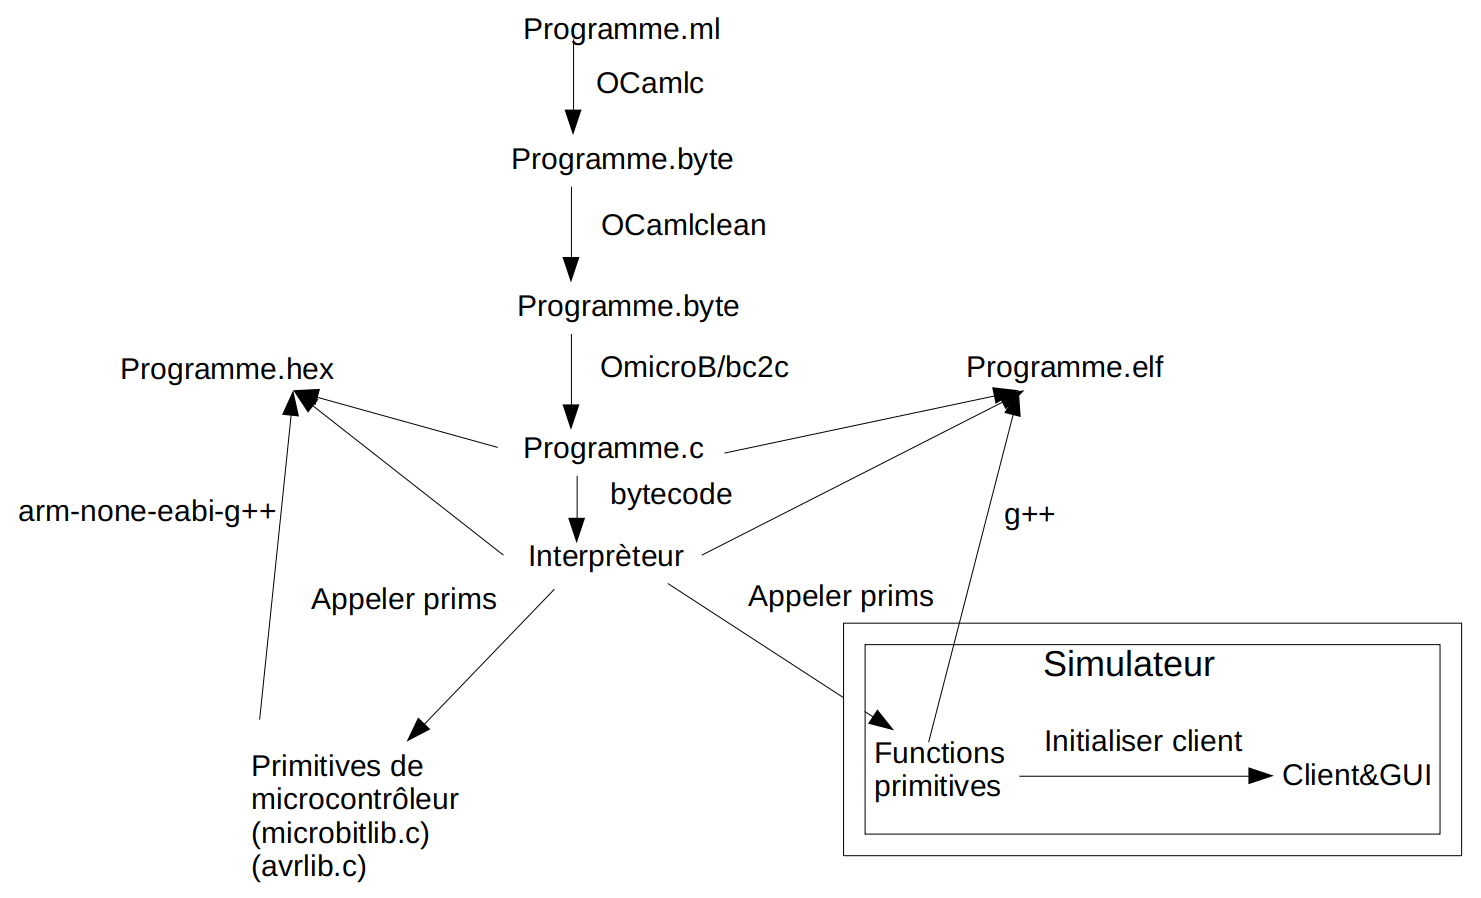
\includegraphics[width=\textwidth]{StructureProgramme.png}\\[1cm]
Cet image montre chaque étape de compilation d'un programme OCaml par OMicroB.
\begin{enumerate}
	\item \textbf{ocamlc} compile le fichier \textbf{.ml} avec la bibliothèque et génére un fichier \textbf{.byte}.
	\item \textbf{ocamlclean} traite le fichier généré \textbf{.byte}.
	\item \textbf{bc2c} est le compilateur de \textbf{OMicroB}, il permet de transférer le code binaire à un programme \textbf{.c}.
	\item \textbf{g++} compile le \textbf{programme.c} et la bibliothèque de simulateur \textbf{sf-regs} puis génère le fichier exécutable \textbf{.elf}.
	\item \textbf{arm-none-eabi-g++} compile le \textbf{programme.c} avec la bibliothèque de microcontrôleur (avrlib, microbitlib, etc) puis génére le fichier exécutable \textbf{.hex}.\\
\end{enumerate}

\textbf{OMicroB} produit deux fichiers exécutables après de compiler un programme \textbf{OCaml}.

- \textbf{.elf} est exécutable en mode simulation, il permet de démarrer le simulateur et montrer le changement des états de pin et les effets de programme sur une interface graphique.\\
- \textbf{.hex} est exécutable sur un microcontrôleur.

\clearpage
\pagestyle{fancy}
\lhead{Simulateur}
\rhead{\thepage}
\fancyfoot{}
\section{Simulateur}
Pour afficher les effets de programme exécuté sur un microcontrôleur, on propose un simulateur qui sert à afficher simultanément l'état de chaque pin et chaque composant pendant l'exécution du programme. Donc on peut considérer l'interprèteur de \textbf{OMicroB} comme un producteur qui produit les demandes de visualisation. La simulateur est un consommateur, il satisfait chaque demande en visualisant les effets sur une interface graphique. Donc on peut implémenter un architecture \textbf{producteur-consommateur} pour réaliser le simulateur, un producteur transfère les demandes de l'interprèteur au consommateur, le consommateur visualise sur l'interface graphique finalement.\\

Considérons la facilité du développement, nous séparons la simulateur en deux parties indépendantes, \textbf{serveur} et \textbf{client}, le serveur est producteur et client est consommateur. Ses avantages est que:
\begin{enumerate}
	\item Séparer le logiciel en deux parties indépendantes, nous pouvons développer paralèllement, c'est plus facile de travailler en groupe.
	\item On peut mieux maintenir la simulateur. Lorsqu'il y a des erreurs générées pendant l'exécution, il plus pratique de localiser où produit l'erreur.
\end{enumerate}

Par conséquence, on a un simulateur dont la structure est décrite par cette image, il exécute deux processus en concurrence. Chaque processus exécute plusieurs threads et travaillent asynchroniquement.

\begin{figure}[htbp]
	\subfigure[la structure de simulateur]{
		\begin{minipage}[t]{\linewidth}
			\centering
			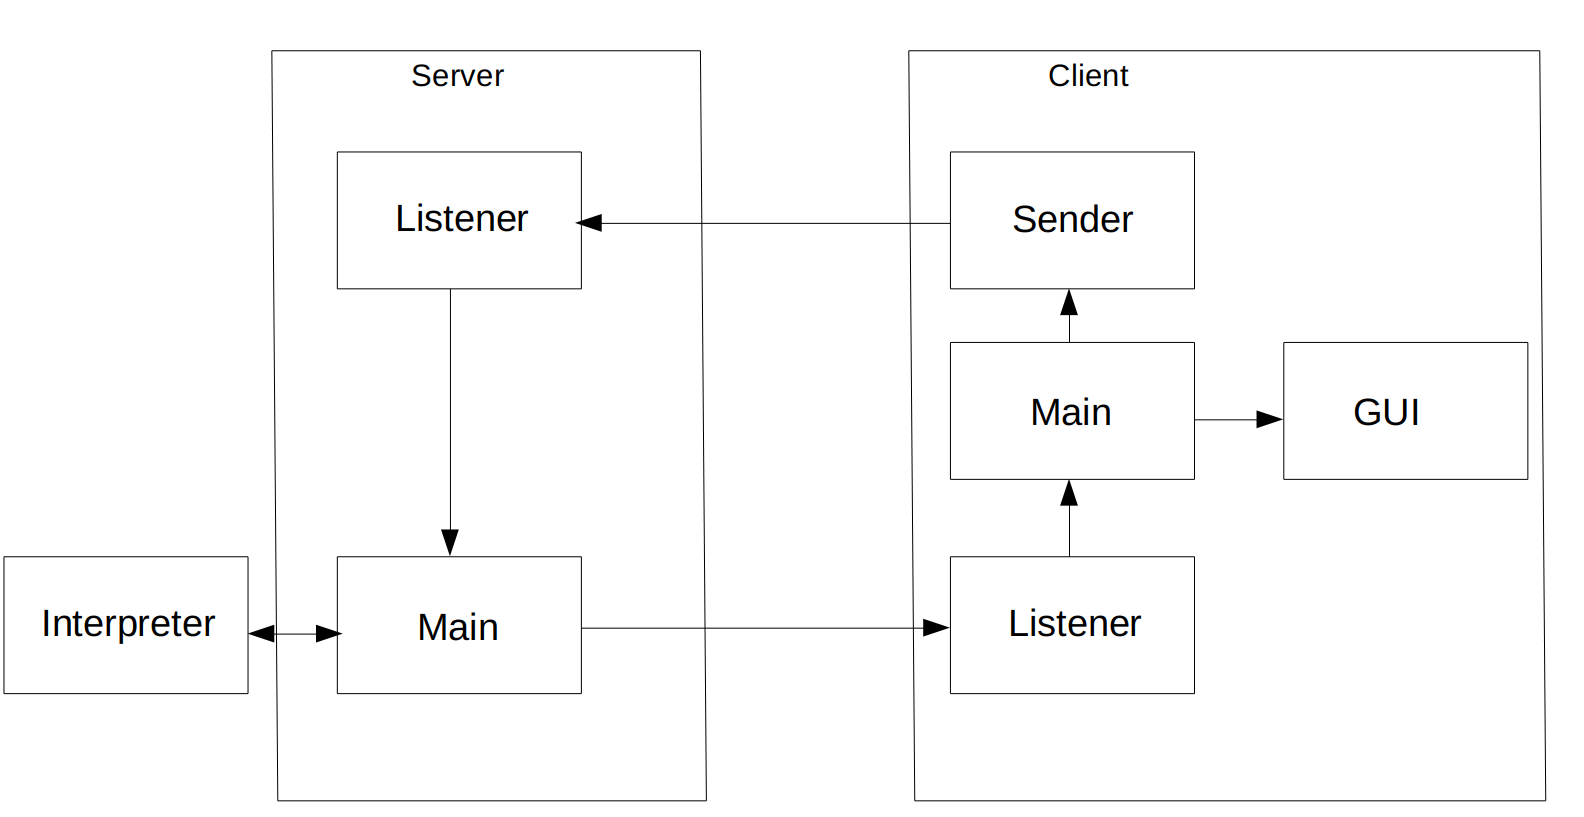
\includegraphics[width=\textwidth]{Simulator.png}
			%\caption{fig1}
		\end{minipage}%
	}%
\end{figure}
\subsection{Serveur}
La partie serveur est codée en C dans "/src/byterun/", il contient des fichiers:
\begin{enumerate}
	\item \textbf{/src/byterun/vm}.
	Ce dossier contient les fichiers de l'interprèteur d'OMicroB, il à été réalisé en OMicroB existant. par exemple le format des type basiques de données, le garbage collector de machine virtuelle ainsi que les définition des instructions de code binaire. Il exécute le programme OCaml et envoie les instructions des codes binaires au serveur.

	\item \textbf{/src/byterun/simul/sf-regs.c/.h}.
	C'est la bibliothèque des primitives de simulateur, la simulateur propose beaucoup d'API aux programmeurs d'OCaml. Ils peuvent appeler ces API dans un programme OCaml qui exécute sur un microcontrôleur, par exemple \textbf{set\_pixel 0 0 true} sert à allumer un LED de microbit. Lorsque ce API est utilisé, la fonction définite dans sf-regs.c est appelé. Elle envoie une instruction au client, puis le client allume LED sur l'interface graphique.

	\item \textbf{src/byterun/shared.c/.h}.
	Ce fichier définit des structures de données partagées entre le processus client et serveur, elles sont stockées dans une mémoire partagée au fur et mesure de l'exécution de programme.
\end{enumerate}
\textbf{Processus Serveur} exécute deux threads, \textbf{listener} et \textbf{Main}.
\begin{enumerate}
	\item \textbf{Main} traite simplement l'instruction qui vient de l'interprèteur et l'envoyer au thread \textbf{listener} de client.
	\item \textbf{listener} reçoit l'instruction venant de \textbf{Sender} et informe \textbf{Main}.
\end{enumerate}


\subsection{Client}
La partie client est programmée en C dans \textbf{src/byterun/client}, se compose de deux fichiers.
\begin{enumerate}
	\item \textbf{client.c} définit les fonctions du travail par exemple traiter le message qui vient du côté serveur.

	\item \textbf{gui.c} implémente l'interface graphique par \textbf{gtk3.0}.
	il nous montre un UI de simulateur permet d'afficher le résultat de programme et les états des Pins pendant la simulation, ainsi que l'interaction par les boutons.\\
\end{enumerate}

\textbf{Processus Client} lance simultanément quatre threads, \textbf{Main}, \textbf{GUI}, \textbf{Sender} et \textbf{listener}.
\begin{enumerate}
	\item \textbf{Main} est le premier thread principal, il traite les arguments venant de processus serveur et connecte aux mémoires partagés, par exemple la mémoire partagée pour la communication et pour le montage. Il est responsable d'exécuter les autres threads.
	\item \textbf{GUI} crée les composants de l'interface graphique en fonction de l'information du montage. Il actualise l'interface dans un boucle infini afin d'afficher le changement des états de chaque composant simultanément.
	\item \textbf{Sender} sert à traiter input de l'utilisateur et envoyer l'instruction au serveur, par exemple appuyer les boutons.
	\item \textbf{listener} reçoit l'instruction venant de serveur, en plus manipuler les composants de l'interface graphique en fonction de l'instruction.
\end{enumerate}


\subsection{Montage}
Pour démarrer le processus client et implémenter l'interface graphique, le client a besoin de savoir quels composants du microcontrôleur il doit afficher sur l'interface graphique. Donc
nous devons proposer un fichier \textbf{circuit.txt} qui décrit les composants du microcontrôleur et les associations entre chaque composant et les Pins correspondants. Avant de démarrer le processus client, le processus analyse est exécuté pour évaluer ce fichier. Une structure qui contient ces informations est stockée dans une mémoire partagée après l'évaluation. Le client peut recevoir les informations des composants du microcontrôleur depuis cette mémoire partagée.\\
Cette fonctionnalité est réalisée dans le dossier \textbf{src/byterun/montage}, la structure est définie dans \textbf{src/byterun/simul/share.h}.


\section{Mécanisme de communication}
\subsection{Protocole de communication}
Pour décrire bien l'instruction, on a implémenté le protocole en plusieurs versions diverses. (S -> C) représente la direction de l'envoie est du serveur au client, (C -> S) est la direction inversée.

\subsubsection{Chaine de caractère} 
Dans la version de protocole initiale, Nous avons choisi la chaine de caractère comme le type du protocole. La raison est que c'est plus pratique de les afficher sur le terminal, on peut facilement vérifier si le protocole est correct pour chaque instruction. \\
La structure du protocole est (\textbf{numéro de primitive, argument1, argument2, .....}).
Pour cette version, nous avons réalisé les protocoles.
\begin{enumerate}
	\item \textbf{PRINT\_IMAGE}: (0, 25 carcatères de 0 ou 1)\\
	(S -> C) Il sert à afficher une image en fonction de 25 caractères, chaque caractère représente l'état de LED. Envoyé par \textbf{microbit\_print\_image(char* ima)}.
	\item[-] \textbf{SET\_PIXEL(x,y,val)}: (1, x, y, val)\\
	(S -> C) Modifier l'état du pixel des coordonnées x et y à val, envoyé par \textbf{microbit\_write\_pixel(int x, int y, int val)}.
	\item[-] \textbf{CLEAR\_SCREEN}: (2)\\
	(S -> C) Mettre les états de tous les pixels à 0, envoyé par \textbf{microbit\_clean\_screen()}.
	\item[-] \textbf{SET\_PIN(p,n)}: (3, numéro de pin, niveau)\\
	(S -> C) Modifier le pin p au niveau n. (n = 0 ou 1), envoyé par \textbf{microbit\_digital\_write}.
	\item[-] \textbf{WRITE\_PIN(p,v)}: (5, p, v)\\
	(S -> C) Modifier le pin p à la valeur v (0 <= v <= 1024), envoyé par \textbf{microbit\_analog\_write}.\\
	
	\item[-] \textbf{INVERSE\_PIN(p,n)}: (0, p)\\
	(C -> S) Inverser l'état de pin qui associéte avec un bouton, lorsque l'utilisateur appuie sur un bouton, ce protocole est envoyé au serveur et \textbf{serveur listener} inverse l'état de pin correspondant. 
\end{enumerate}

\subsubsection{Entier de 32 bits}
Après tester tous les primitives, on est sûr que le protocole est correctement décrite chaque instruction. On commence d'améliorer ce protocole, parceque la formalisation et décodage du protocole consomment beaucoup de temps, ainsi que la chaine de caractère consomment aussi l'espace de mémoire.\\
Commme un integer du langage C se compose de 32 bits, ainsi que 32 bits pour le protocole est suffisant sauf pour PRINT\_IMAGE. Il ne suffit pas à afficher une image dont le nombre de pixel est supérieur à 31. Donc on supprime ce protocole dans cette version, et on réalise la primitive \textbf{microbit\_print\_image(char* ima)} en utilisant le protocole \textbf{SET\_PIXEL(x,y,val)}, il ne suffit d'envoyer le nombre de pixel fois le protocole \textbf{SET\_PIXEL(x,y,val)}.

Par conséquence, la structure du nouveau protocole est \textbf{(numéro de méthode 7bits) :: arguments(25 bits)}.\\
7 bits pour le numéro de fonction, on peut étendre jusqu'à 128 primitives maximum, c'est très suffisant. \\ 25 bits suffit de représenter tous les arguments pour l'instant.
Il y à des protocoles comme ci-dessous
\begin{enumerate}
	\item[-] \textbf{SET\_PIXEL(x,y,val)}: 1(7bits)::x(12 bits)::y(12 bits)::val(1 bits), (S -> C)
	\item[-] \textbf{CLEAR\_SCREEN}: 2(32 bits), (S -> C)
	\item[-] \textbf{SET\_PIN(p,n)}: 3(7 bits)::p(8 bits)::n(17 bits), (S -> C)
	\item[-] \textbf{WRITE\_PIN(p,v)}: 4(7 bits)::p(8 bits)::v(17 bits), (S -> C).\\
	
	\item[-] \textbf{INVERSE\_PIN(p,n)}: 0(7 bits)::p(25 bits) (C->S).
\end{enumerate}


\subsection{Synchronization}
Deux processus exécutent en concurrence, le plus important est que comment synchroniser leur tâche? Nous avons testé le simulateur sans synchronization, et nous avons observé qu'il y a des protocoles qui ne sont pas visualisées sur l'interface graphique. C'est parceque la visualisation de quelques protocoles prend du temps. Par exemple éteindre tous les LEDs ou afficher une image. Donc on a implémenté un mécanisme de communication, il sert à garantir que chaque protocle peut être bien visualisée. Ce sont les étapes pour la communication entre le processus serveur et client.

\textbf{Etapes pour afficher d'un protocole}
\begin{enumerate}
	\item \textbf{Client listener} attend le protocole de serveur.
	\item \textbf{Server main} vérifie si le protocole précédente est bien visualisé.\\
	- Si oui, il envoie la nouveau protocole au client.\\
	- Sinon, \textbf{Server main} attend .
	\item \textbf{Server main} réveille le thread \textbf{client listener}.
	\item \textbf{Client listener} vérifie si la nouvelle instruction arrive.\\
	- Si oui, il informe au \textbf{GUI} afin d'afficher le nouvel état de composant.\\
	- Sinon, c'est un déblocage fausse, il continue à attendre.
	\item \textbf{Client listener} réveille le thread \textbf{server main}.
	\item retour à l'étape 1.
\end{enumerate}

Pour garantir que ces deux processus exécutent étape par étpae. Nous avons essayé plusieurs manières diverses au fur et mesure du développement.

\subsubsection{Pipe + Signal}
Au début, nous utilisions le pipe et le signal pour transmettre l'instruction. Pour la direction du serveur au client, le protocole est transmis par le pipe, et la direction inverse, on a utilisé le signal pour représenter le protocole, parce qu'il n'y a que événements, soit appuyer le bouton A soit le boutton B, donc on a attaché deux signaux SIGUSR1 et SIGUSR2 au ces deux bouttons, si le boutton est appuyé, le serveur reçoit SIGUSR1 ou SIGUSR2, et la fonction \textbf{handler} inverse l'état de pin correspondant.

Son avantage est que l'on n'a plus besoin exécuter un thread \textbf{listener} dans le processus \textbf{serveur}. Comme la fonction \textbf{handler} exécute dès que le processus serveur reçoit le sigal depuis le processus client. 

Mais le mécanisme de signal est très limité, le signal utilisable est divers pour le système différent, par exemple pour linux on a droit d'utiliser les signaux qui sont supérieur à 32, mais pour macOS, il y a seulement quatres signaux qu'on peut utiliser.

\subsubsection{Pipe}
Après qu'on a constaté la limite du signal, on a essayé d'utiliser deux pipes pour la communication en deux direction. Pipe possède le mécanisme de protection, et il peut  synchroniser automatiquement la communication, mais il 	génère un fichier temporaire pour la lecture et l'écriture, ainsi que il est moins efficace que la mémoire partagée. Donc on a finalement décidé d'utiliser la mémoire partagée.

\subsubsection{Mémoire partagée}
La mémoire partagée sert à communiquer entre le serveur et client, puisque c'est la plus rapide manière du transport de données. Mais son inconvénient est que l'on doit implémenter un mécanisme de synchronization afin de protéger les données partagées pour la lecture et l'écriture. Donc pour deux directions du transport (du serveur au client et du client au serveur), on a besoin de deux mémoires partagées, \textbf{shm1} est écrit par le serveur, le client le lit. \textbf{shm2} est inversé.\\

Afin de synchroniser la lecture et l'écriture, on met un mutex et une variable conditionnelle pour chaque mémoire partagée. Il garant que chaque instruction de serveur peut être bien traiter.\\




\clearpage
\section{Méthodologie de réalisation}
Selon ce qui précède, notre objectif est de simuler les informations d'entrée et de sortie du micro-controlleur monopuce, pour réaliser les fonctionnalité du simulateur, il y a deux versions, en \textbf{haut niveau} et en \textbf{bas niveau}.

\subsection{Version haut niveau}
\textbf{haut niveau} est que l'on simule abstraitement un microcontrôleur, la simulation haut niveau ne reflète pas les intéractions réelles entre le microcontrôleur et son environement. On implémente les tableau pour stocker les états de chaque composant. Dès que l'état de composant est modifié par la primitive, on modifie le tableau directement.\\
Par exemple le serveur appelle la primitive \textbf{microbit\_write\_pixel 0 0 true}, il ne suffit de modifier le tableau qui stock l'état des LEDs. pixels[0][0] = true.\\

\textbf{Avantage}\\
La version est plus simple, il a juste besoin de modifier le tableau correspondant.\\

\textbf{Inconvénient}\\
Cette méthode n'est pas générale, parce que les composants sont différents pour les microcontôleurs divers, on ne peut pas implémenter les tableau pour chaque microcontrôleur.
Si le microcontrôleurs se change, nous devons réimplémenter le protocole et les tableaux des composants.


\subsection{Version bas niveau}
\textbf{bas niveau} est que l'on simule réellement un microcontrôleur, afin de mieux simuler l'état de fonctionnement réel du microcontrôleur à partir de l'architecture du microcontrôleur, nous espérons modifier directement l'état du \textbf{tableau de pins}, sans avoir besoin d'autres appels de fonctions, et refléter directement les effets de ces modifications sur \textbf{l'interface graphique}. Cela fera quelques changements basés sur le haut niveau précédent.

Lorsque nous voulons allumer un led, nous devons d'abord chercher son \textbf{pin\_row} et \textbf{pin\_col} correspondant, puis mettons \textbf{pin\_row} à haut niveau et \textbf{pin\_col} à bas niveau.\\

\textbf{Avantage}
La simulateur de bas niveau peut s'adapter à un grand nomrbe de composants électroniques externes au microcontrôleur puisque les interactions sont réalisées par la modification des états des pins. Donc le protocole \textbf{SET\_PIN} est général pour le plupart des primitives, on n'a plus besoin de protocle spécifique comme \textbf{SET\_PIXEL}. Même si le microcontôleur branche un composant spécifique, par exemple le moteur, l'écran LCD, etc, on a juste besoin de changer un fichier du montage, et rajouter un protocole spécifique mais pas tout le simulateur.\\

\textbf{Inconvénient}
Le traitement d'une instruction est plus compliqué, l'interaction entre le serveur et le client est plus fréquente.\\
Par exemple, pour allumer un \textbf{LED}, le serveur envoie une seule instruction \textbf{SET\_PIXEL(X,Y,True)} au client dans la version haut niveau. Mais dans le bas niveau, le serveur doit d'abord chercher le \textbf{pin\_row} et \textbf{pin\_col}, puis envoyer deux instructions \textbf{SET\_PIN(pin\_row, 1)} et \textbf{SET\_PIN(pin\_col, 0)} au client.

\clearpage


\section{Fonctionalités Implémentées}
\subsection{Visualiser du texte sur la matrice des leds}
Tout d'abord,nous convertissons les informations de chaque caractère en forme des graphiques raster dans une table en code hexadécimal 5x8 bits en bien tirer par order du code ASCII.Lorsqu'on recevoir un command d'imprimer une caractère à l'écran,
on va calculer ASCII code correspond à cette caractère,et puis en fonction de ce ASCII code ,on peut calculer le décalage dans la table de code hexadécimal correspond à cette caractère. Sortir enfin les 5 * 8 bits d'information dont il dispose. Prendre 5 * 5 bits d'entre eux et les imprimer pixel par pixel sur l'écran.\\

Une exemple de visualiser la caractère 'A' sur la matrice des leds.
\begin{enumerate}
	\item calcule le code ASCII de 'A', c'est 65.
	\item calcule son décalage c'est 65 * 5 = 325.(parce que l'écran est de 5 lignes et chaque ligne est composé de 2 chiffre hexadécimal)
	\item cherche son table de code hexadécimal correspondant dans le tableau, c'est \{30,28,38,28,28\}.
	\item nous convertissons code hexadécimal en forme code binaire.\\
	00110000\\
	00101000\\
	00111000\\
	00101000\\
	00101000\\
	\item modifier les Pins de chaque LED en fonction de cette code binaire. On a finalement une image comme cela.\\
	\centering
	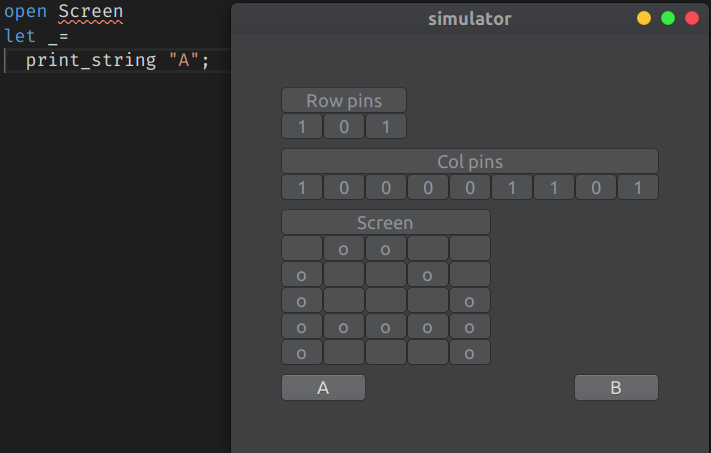
\includegraphics[width=0.6\textwidth]{printA.png}\\[1cm]

\end{enumerate}

\clearpage

\subsection{Analyser le ficher du montage}
Pour le montage de microcontrôleur, il a besoin d'un fichier qui stocke les informations de chaque composant de microcontrôleur comme le nombre des pins, les association entre chaque composant et le pin correspondant. Une fois que le simulateur connait ces informations, il peut implémenter l'interface graphique et contrôler les composants par modifier l'état des pins.\\
Donc on a utilisé Flex, Yacc et langage C afin de réaliser un langage descriptif.
\begin{enumerate}
	\item On défini les \textbf{tokens} dans le fichier \textbf{parser.y}.
	\item Lier les mots prédéfinis avec ces tokens dans \textbf{lexer.lex}
	\item Créer les noeuds de \textbf{AST}(l'arbre d'analyse syntaxe) dans fichier \textbf{AST.c} et \textbf{AST.h}.
	\item Réaliser les fonctions de l'évaluation dans le fichier \textbf{get\_env.c}.
\end{enumerate}

\begin{figure}[htbp]
	\subfigure[cf.exmple \textbf{circuit.txt}]{
		\begin{minipage}[t]{\linewidth}
			\centering
			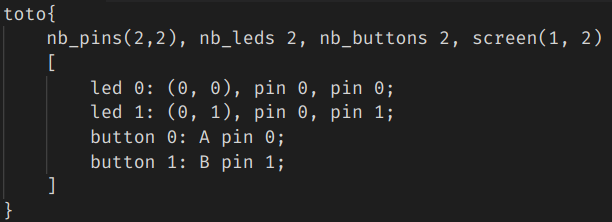
\includegraphics[width=0.5\textwidth]{circuit_ex.png}\\[1cm]
			%\caption{fig1}
		\end{minipage}%
	}%
\end{figure}

\textbf{Le grammaire et les mots prédéfinis}
\begin{enumerate}
	\item \textbf{nom du simulateur\{l'information du montage\}}: C'est la structure du langage.
	\item \textbf{nb\_pins (num\_row, num\_col)}: \textbf{num\_row} est le nombre de pins de ligne(row), \textbf{num\_col} est celui de colonne.
	\item \textbf{nb\_leds num}: \textbf{num} est le nombre de leds.
	\item \textbf{nb\_buttons num}: \textbf{num} est le nombre de buttons.
	\item \textbf{screen(row, col)}: Cela indique le nombre de ligne et colonne de matrice des LEDs.
	\item \textbf{led id: (row, col), pin id1, pin id2}: Cela représente le numéro du LED et ses coordonnées dans la matrice, ainsi que l'association entre le led et deux pins correspondant. id1 est l'identifiant de pin row, id2 est celui de pin col.
	\item \textbf{button id: étiquette pin id}: Cette une déclaration du bouton dont l'identifiant est id et son étiquette, ainsi que le pin correspondant.
\end{enumerate}

\clearpage
\pagestyle{fancy}
\lhead{Méthodologie de réalisation}
\rhead{\thepage}
\fancyfoot{}

\clearpage



\section{Scénarios et Tests}
Ce sont les étapes de simuler un programme ocaml par la simulateur du microbit.
\begin{enumerate}
	\item Charger l'information du montage par un fichier \textbf{circuit.txt}.
	\item Le processus montage analyse ce fichier et génère une structure du montage, en plus envoie au serveur et au client par le mémoire partagée \textbf{envid}.
	\item Le processus client implémente une interface graphique en fonction de structure du montage.
	\begin{figure}[htbp]
		\centering
		\subfigure[la description du circuit]{
			\begin{minipage}[t]{0.4\linewidth}
				\centering
				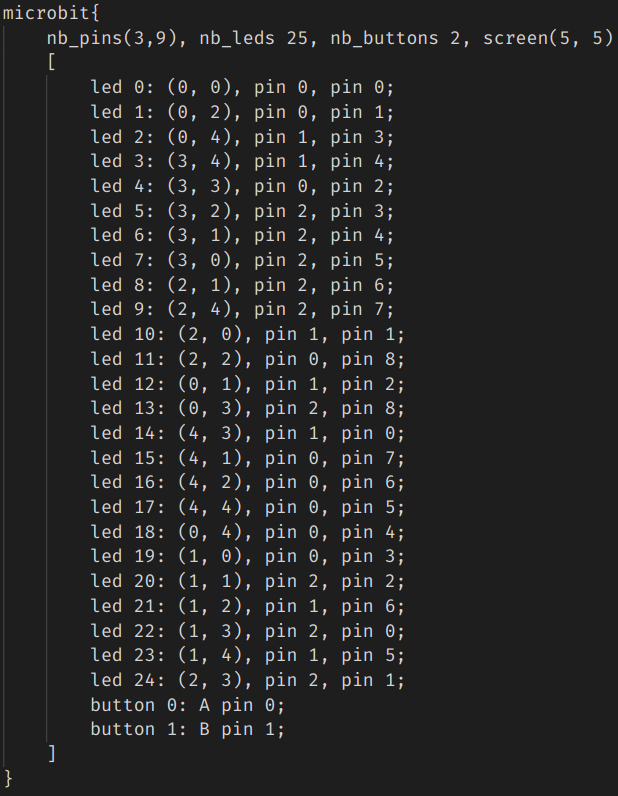
\includegraphics[width=\textwidth]{circuit.png}
			\end{minipage}%
		}%
		\subfigure[l'interface graphique de microbit]{
			\begin{minipage}[t]{0.4\linewidth}
				\centering
				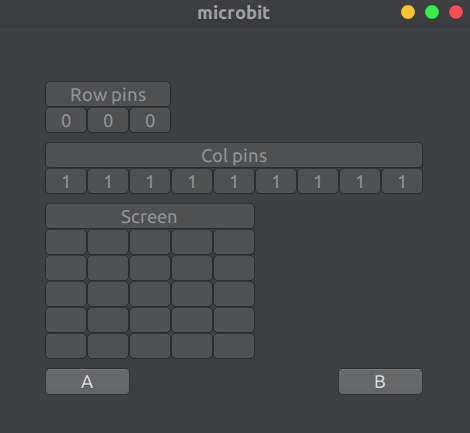
\includegraphics[width=\textwidth]{gui.png}
			\end{minipage}%
		}%
		\centering
	\end{figure}
	\item Le serveur interprète le programme OCaml, puis envoie des protocoles au client.
	\item Le client visualise les effets du programme.
	\begin{figure}[htbp]
		\centering
		\subfigure[un programme ocaml]{
			\begin{minipage}[t]{0.3\linewidth}
				\centering
				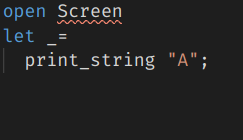
\includegraphics[width=\textwidth]{printAprog.png}
			\end{minipage}%
		}%
		\subfigure[L'effet de la visualisation]{
			\begin{minipage}[t]{0.3\linewidth}
				\centering
				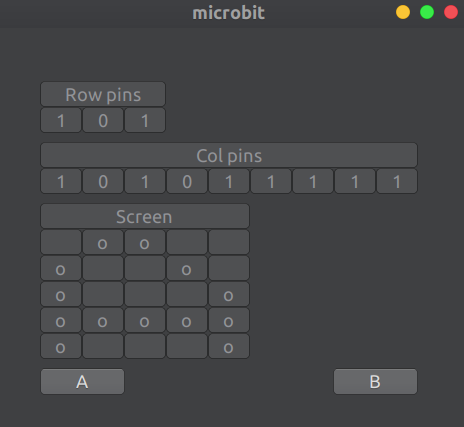
\includegraphics[width=\textwidth]{printAeffets.png}
			\end{minipage}%
		}%
		\centering
	\end{figure}

\end{enumerate}
\clearpage

\section{Problème et Solution}
\subsection{Choix de processus ou de thread}
Quand on désigne l'architecture du simulateur, on a deux choix pour le côté du serveur et client. Soit on les sépare en deux threads, soit deux processus. Les avantages du thread est que c'est plus facile de partager les données et réaliser la synchronization. Néanmoins, la partie serveur est compilé par \textbf{ocamlc} dans une étape de la compilation, et nous utilisons \textbf{gtk+3.0} pour réaliser l'interface graphique, le compilateur \textbf{ocamlc} ne peut pas compiler la bibliothèque de \textbf{gtk+3.0}, donc on sépare le serveur et le client en deux processus.


\subsection{Synchronization}
Comme ce que l'on a présenté, le serveur envoie les protocoles au client, et le client visualise simultanément les états de chaque composant, mais pour quelque protocole par exemple \textbf{CLEARSCREEN}, il prend du temps parce qu'il faut éteindre tous les LEDs. Donc s'il n'y a pas de mécanisme de synchronization afin de garantir que le nouveau protocole arrive après le traitement du protocole précédent, il risque de perdre quelques instructions.

Pour synchroniser le transfert du protocole entre le serveur et le client, nous avons essayé plusieurs méthodes 


\clearpage

\subsection{Problème de conflit}
\begin{figure}[htbp]
	\subfigure[cf.le circuit réel de microbit]{
		\begin{minipage}[t]{\linewidth}
			\centering
			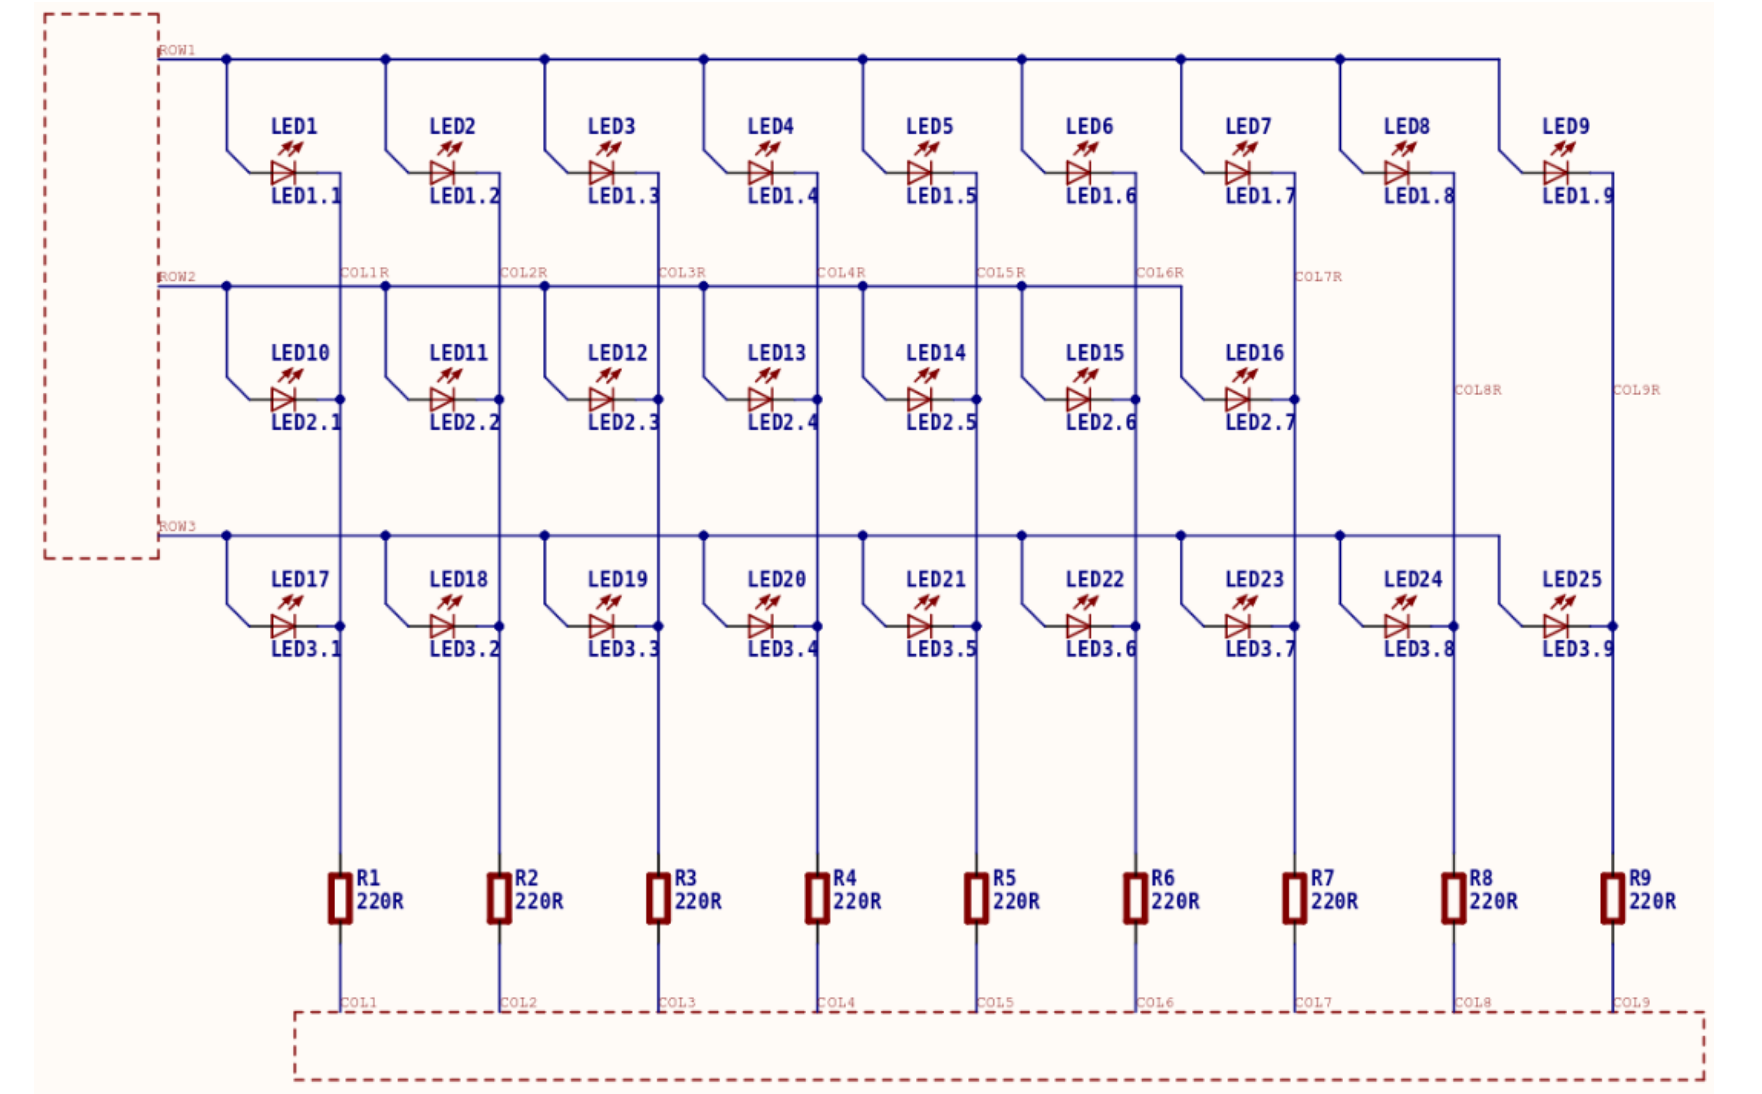
\includegraphics[width=0.8\textwidth]{circuitReelMicrobit.png}
		\end{minipage}%
	}%
\end{figure}
Cet image montre le circuit du \textbf{microbit}, la matrice de LED se compose d'une matrice de pins de 3 * 9. Pour allumer un LED, on doit mettre le \textbf{pin\_row} correspondant au niveau \textbf{HIGH}, et mettre son \textbf{pin\_col} au niveau \textbf{LOW}.

\begin{figure}[htbp]
	\subfigure[cf.le tableau des associations entre le LED et les pins correspondant]{
		\begin{minipage}[t]{\linewidth}
			\centering
			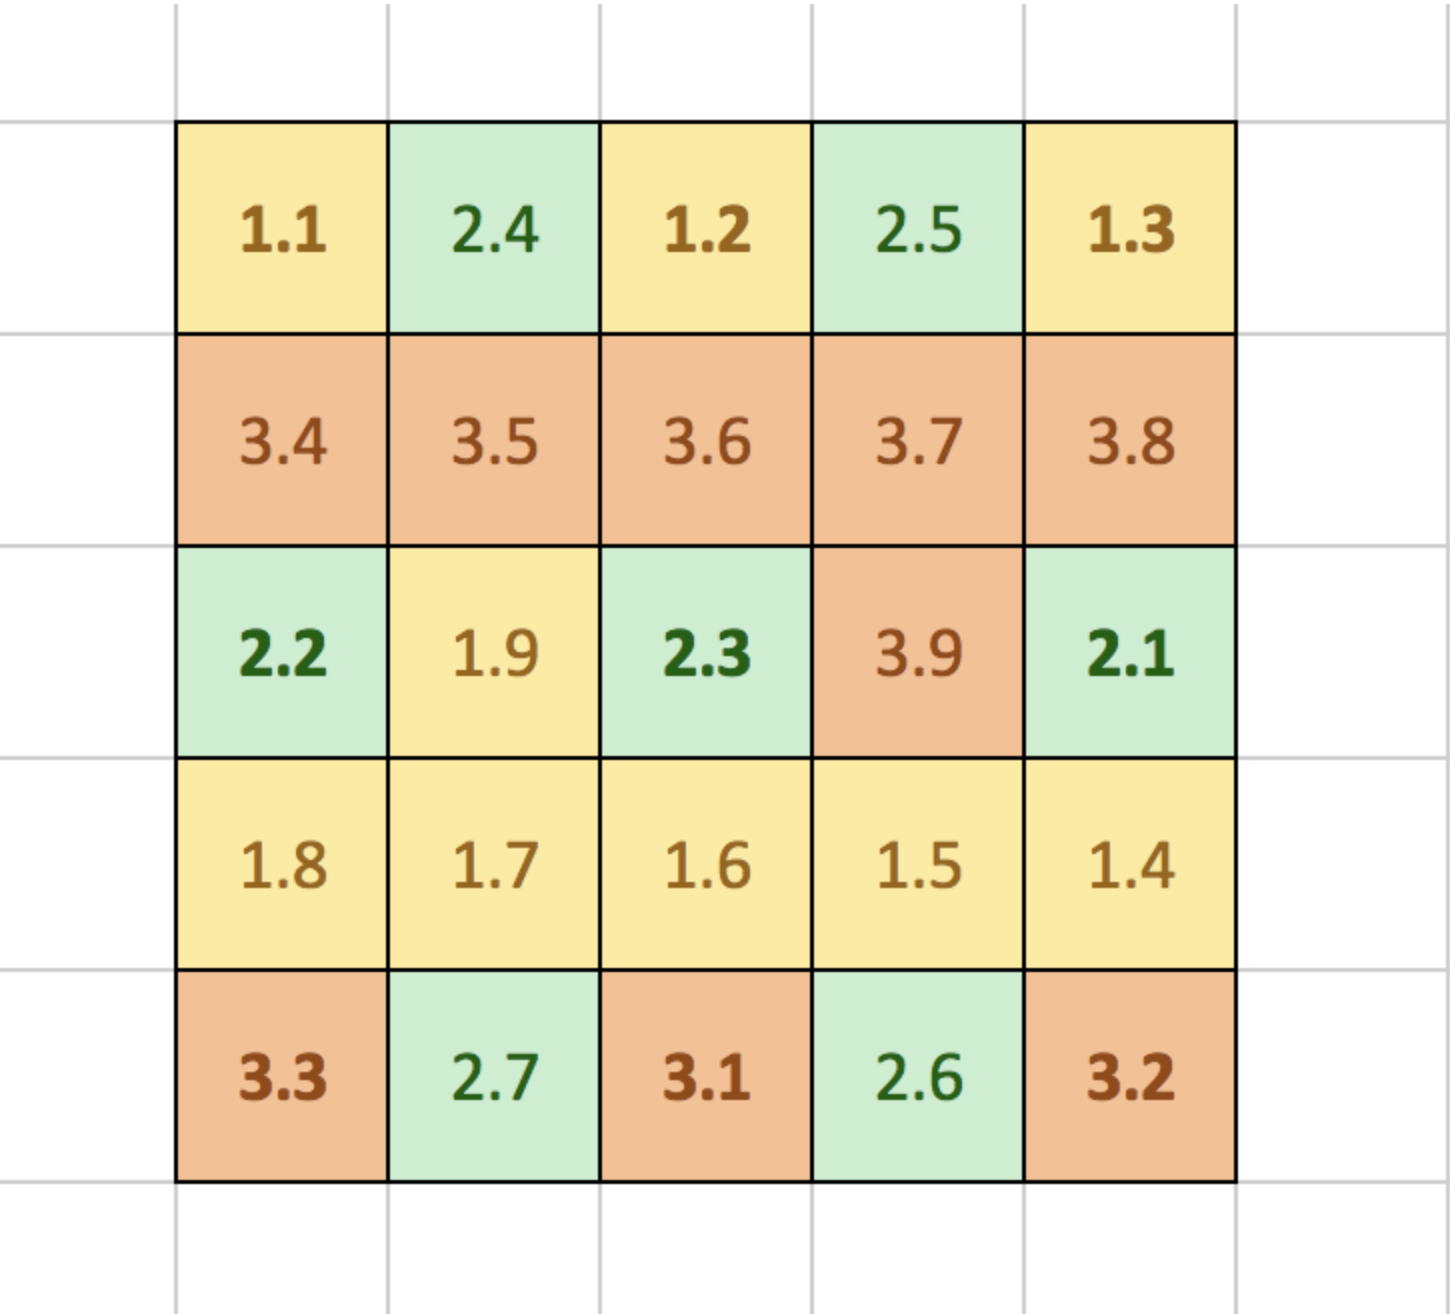
\includegraphics[width=0.3\textwidth]{matrice_Pins.png}
			%\caption{fig1}
		\end{minipage}%
	}%
\end{figure}
Ce tableau montre la relation de position entre le circuit du  \textbf{microbit} et l'éran du \textbf{microbit}.
\clearpage
Lorsque nous voulons allumer un seulement LED, il n'y a pas de conflit. Par exemple, pour \textbf{LED 0 0}, on met \textbf{pin\_row1} au niveau \textbf{HIGH}, et \textbf{pin\_col1} au niveau \textbf{LOW}. Les effets de la simulation est comme cet image.\\
\begin{figure}[htbp]
	\subfigure[cf.exmple \textbf{allumer LED 0 0}]{
		\begin{minipage}[t]{\linewidth}
			\centering
			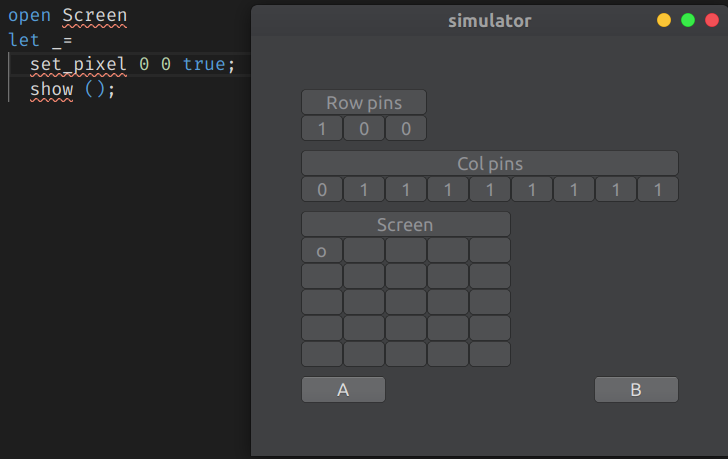
\includegraphics[width=0.5\textwidth]{no-conflict.png}\\[1cm]
			%\caption{fig1}
		\end{minipage}%
	}%
\end{figure}\\

Néanmoins, si on veut allumer deux LEDs dont le pin\_row n'est pas la même, il y aura le conflit. Par exemple on allume \textbf{LED 0 0} et \textbf{LED 0 1}. On doit mettre \textbf{pin\_row1} et \textbf{pin\_row3} au niveau \textbf{HIGH}, mettre \textbf{pin\_col1} et \textbf{pin\_col4} au niveau \textbf{LOW}. Dans ce cas-là, il y aura quatre LEDs allumé.
\begin{enumerate}
	\item \textbf{LED 0 0} correspondant à \textbf{pin\_row1, pin\_col1}.
	\item \textbf{LED 4 3} correspondant à \textbf{pin\_row1, pin\_col4}.
	\item \textbf{LED 0 1} correspondant à \textbf{pin\_row3, pin\_col4}.
	\item \textbf{LED 2 4} correspondant à \textbf{pin\_row3, pin\_col1}.
\end{enumerate}
\begin{figure}[htbp]
	\subfigure[cf.exmple \textbf{allumer LED 0 0 et LED 0 1}]{
		\begin{minipage}[t]{\linewidth}
			\centering
			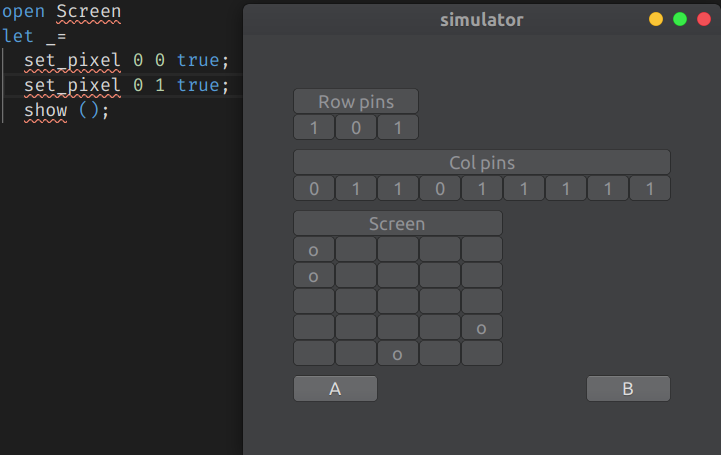
\includegraphics[width=0.5\textwidth]{conflit.png}\\[1cm]
			%\caption{fig1}
		\end{minipage}%
	}%
\end{figure}



\end{document}
